\section{VM-centric Snapshot Deduplication}
\label{sect:dedupe}
%snapshot representation

%We use the The deduplication process is first conducted among snapshots within each VM
%and then is conducted across VMs.
%Given the concern that searching duplicates across VMs is a global feature which can affect parallel performance
%and complicate failure management,
%we only eliminate the duplication of a small but popular data set while still maintaining a cost-effective deduplication ratio.
%For this purpose, we exploit the data characteristics of snapshots and collect most popular data.
%Data sharing across VMs is limited within this small data set such that adding replicas for it could enhance fault tolerance

%A deduplication scheme compares the fingerprints of the current snapshot
%with its parent snapshot and also other snapshots in the entire cloud.
%The traditional approach compares all fingerprints and 
%stores one copy for all of a chunk's duplicates.
%We call this as  the VM-oblivious (VO) approach.
Our VC design has the following  objectives: 1)  localizing deduplication while identifying a decent amount of
duplicates among VMs to maintain a competitive deduplication efficiency and simplify snapshot management;
2) Minimizing the number of file system blocks shared among VMs and adding extra replicas for shared blocks.

\comments{
\begin{itemize}
\item
1) Localize the deduplication and data blocking within each VM as much as possible so 
that any failure of a file system block mainly affects the associated VM.
Localizing the snapshot data deduplication within a VM
improves the system by increasing data independence between different VM backups,
simplifying snapshot management and statistics collection,
and facilitating parallel execution of snapshot operations.
\item
2) Maintain a competitive deduplication efficiency while being resource-friendly to other
existing cloud services.
Cross-VM duplication can be desirable since  there are many cloud images
use widely-used software and libraries and their data blocks are duplicate. 
As the result, different VMs tend to backup large amount of highly similar data.
\item
\end{itemize}
}
\subsection{Key VM-centric  Strategies}
\label{sect:vc-strategies}

%Inner-VM duplication can be very effective within VM's snapshots. There
%are typically a large number of duplicates existing among the snapshots
%for a single VM.  

%Our multi-level pipeline process can minimize 
%the cost of deduplication while maximize the its efficiency at each level,
%and it is parallel since each segment is processed independently.

%Our VC differentiates duplicates within a VM and cross VMs,
%and conducts \textit{Inner-VM} and \textit{cross-VM} detection separately. 

\begin{itemize}
\item \textbf{VM-specific local duplicate search within similar segments.}
We start with the standard dirty bit approach in a coarse grain segment level.
In our implementation with Xen at an Alibaba platform, the segment size is 2MB
and  the device driver is extended to support  changed block tracking. 
Since every write for a segment will touch a dirty bit, the device driver maintains dirty bits in memory
and cannot afford a small segment  size.
%Xen doesn't directly support it, However, their open-source 
%architecture allows anyone to extend 
%and use the  Xen virtual device driver to implement a feature called ``changed block tracking''
%for the storage device and the dirty bit setting is maintained in a coarse grain level we call it a segment.
It should be noted that dirtybit tracking is supported or can be easily implemented in 
major virtualization solution vendors. For example,
%(VMware, Xen, Microsoft).  
%VMware support it directly; 
the VMWare hypervisor has an API to let external backup applications know 
the changed areas since last backup. 
%We implement dirty bit tracking this way in Alibaba's platform.  
The Microsoft SDK provides an API that allows external applications to monitor 
the VM's I/O traffic and implement  the changed block tracking feature.

Since the best deduplication uses a nonuniform chunk size 
in the average of 4K or 8K~\cite{??},  
%This allows the system to achieve deduplication even when there are insertions/deletions which would
%affect many fixed-size chunks.
we conduct additional local inner-VM deduplication by comparing
dirty segment's chunk fingerprints to similar segments from its parent snapshot. 
For every segment, the minimum value of all its chunk fingerprints is computed during backup
and is recorded in the snapshot recipe.
When we are processing a dirty segment,
we can easily find similar segments from the
parent snapshot recipe and load their segment recipes. Then 
given a set of data chunks within a dirty segement,  we compare  these chunk fingerprints
with those in similar segments.  
For example, with a 2MB segment, there are about 500 fingerprints to compare.
The amount of memory for maintaining those fingerprints in similar segment s is small, as we only
load one dirty segment at a time.


%If we use 4KB in level-1, then such a level-1 should have similar dedup efficiency 
%as the current level-1 and level-2 combined, because finally they equal to comparing  
%parent snapshot at 4KB granularity.
%
%However, at level-3 things are different. If we use 4KB fix-size block uniformly, it would be harder for different VM to share data through PDS, because there is no guarantee that the location of duplicate data on different VM disks are always aligned at 4KB boundary. For example, if two VMs each has a copy of duplicate data, but they are not aligned, then we won't be able to detect them. Our study at the current small data set has shown that using 4KB fix-size block will make PDS method less efficient by nearly 10%. Over the long time, more and more OS variations will co-exist in the cluster, making this 4KB fix-size approach inefficient in reducing duplicate data across VMs.

%\item \textit{Level 2  Chunk fingerprint comparison.}
%If a segment is modified, we perform fine-grained deduplication 
%by comparing the fingerprints of its chunks to the same segment's recipe in the previous snapshot,
%thus eliminate partial data duplication within the segment.
%\end{itemize}
%
%In general, operations at level 1 have almost no cost and most of unmodified data are filtered here. 
%To process a dirty segment at level 2, 
%there requires no more than one DFS access to load the segment recipe from previous snapshot,
%and a tiny amount of memory to hold it in main memory.

\item \textbf{Cross-VM deduplication with popular chunks and replication support}
This step accomplishes the standard global fingerprint  comparison as conducted
in the previous work~\cite{??}.
One key observation is that the inner deduplication has removed many of the duplicates.
There are fewer deduplication opportunities across VMs while the memory and network
consumption for global comparison is more expensive.
Thus our approximation is that the global fingerprint comparison only searches for the top $k$
most popular items. This dataset is called PDS (common data set). 
%Since duplicate sharing patterns among  VM follows a zip-like distribution,  
The popularity of a chunk is the number  of data chunks  from different VMs
that are duplicates of this chunk after the inner VM deduplication.
This number can be computed periodically on a weekly basis.
Once the popularity of all data chunks is collected, the system only maintains the top $k$
most popular chunk signatures in a distributed shared memory.  
%For cross-VM comparison, we only store  top $k$ items and $k$ is chosen to be relatively small.

Since $k$ is relatively small and these top $k$ chunks are shared among multiple VMs, 
we can afford to provide extra replicas for these popular chunks to enhance the fault resilience.
%We will provide an analysis of the space need and fault tolerance in the next subsection.

\item \textbf{VM-centric file system block management.}
When a chunk is not detected as a duplicate to any existing chunk, this chunk will be written
to the file system. Since the backend file system typically uses a large block size such as 64MB, each VM will 
accumulate small local chunks. We manage this accumulation process using an append-store  scheme
and discuss this in details in Section~\ref{sect:arch}.
The system allows all machines conduct the backup in parallel in different machines, and each machine
conducts the backup of one VM at a time, and thus only requires a write  buffer for one VM.

PDS chunks are stored in a separate append-store instance. In this way, each
file block for non-PDS chunks is associated with one VM and does not contain
any PDS chunks. 
\end{itemize}

We have not  adopted the  sampled index~\cite{Guo2011} 
for  popular data chunks and  this is because sampling requires the use of prefetching to be effective.
%For a small set of popular data chunks, the prefetching strategy
%used In the sampled index will not work well because 
For the data sets we have tested, the spatial locality is limited among popular
data chunks and  on average the number of consecutive data chunks is 7 among popular chinks, which is not sufficient.
%to be effective for index sampling.


 \subsection{Impact on deduplication efficiency}
%VM-oriented Fault Isolation}
%Our objective for fault isolation is to minimize the number of VMs affected when there are failures
%in the cluster.  
%The inner-VM deduplication does not depend on any global service and the comparison
%for each VM is localized within the parent and the current snapshot.
%Lack of data dependence between VMs brings 
%Our analysis below will show that the algorithm can still deliver competitive
%deduplication efficiency after making these approximations.
%With cross-VM deduplication, shared data chunks
%create an artificial dependence  among VMs. 
%Thus we only maintain the index for the most popular chunks to reduce the inter-VM dependence
%while still accomplishing competitive deduplication efficiency. 

%The management for popular data chunks contains two aspects.



We analyze how the choice of value  $k$ impacts the deduplication efficiency.
%It also  compares the  fault resilience of our VM-centric deduplication approach with a standand approach using 
%global deduplication.
%\subsubsection{Impact of PDS deduplication}
The analysis is based on the characteristics  of the VM snapshot traces
studied from  Alibaba's production user data.
Our previous study shows that the popularity of data chunks after inner VM deduplication follows 
a Zipf-like distribution\cite{zipf} and its
exponent $\alpha$ is ranged between 0.65  and  0.7.~\cite{ieeecloud}. 
%As a result, it can be proved that deduplication efficiency of PDS index is scalable:
Table~\ref{tab:symbol} lists parameters used in this analysis.


\begin{figure}
\centering
%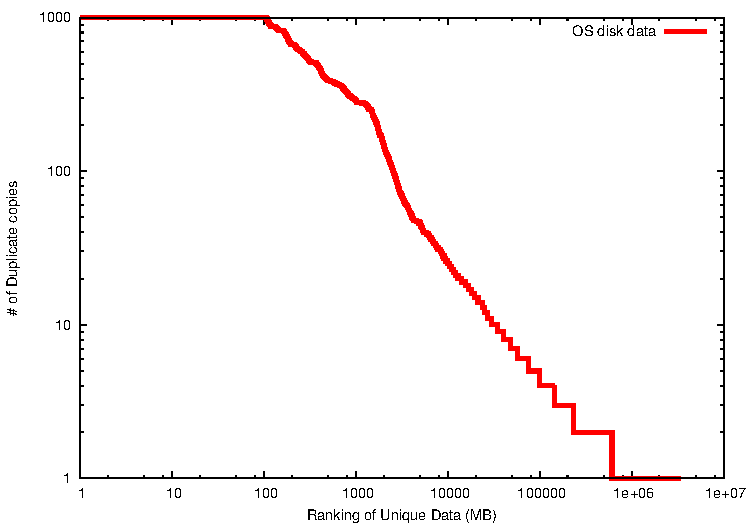
\epsfig{file=log-log.disk,width=3in}
%source ../vm_snapshot_sim/images/log-log.disk.eps
 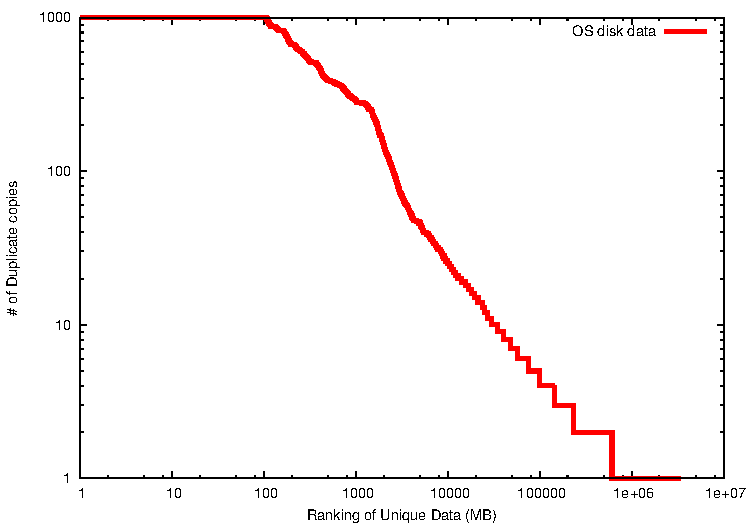
\includegraphics[width=3in]{figures/log-log-disk}
\caption{Duplicate frequency versus  chunk ranking in a log scale.}
\label{fig:Datazipf}
\end{figure}

\begin{table}[ht]
\centering
\begin{tabular}{|p{1.25cm}|p{6.5cm}|}
\hline
$k$ &  the number of top most popular chunks\\ 
\hline
$c$ &  the total amount of data chunks\\ 
\hline
$c_u$ &  the total amount of unique fingerprints after inner VM  deduplication\\
\hline
$f_i$ &  the frequency for the $i$th most popular fingerprint\\
\hline
$\delta$ &  the percentage of duplicates detected in inner VM deduplication\\
\hline
$\sigma$ &  the number of unique non-PDS chunks over  the number of the PDS chunks.\\
\hline
$p$ & the number of machines in the cluster\\
\hline
$V$ & the number of VMs on each machine\\
\hline
$D$ & the amount of unique data on each machine\\
\hline
$C$ & the average data chunk size. Our setting is  4K.\\
\hline
$s$ & the average size of file system blocks in the distributed file system. The default is  64MB.\\
\hline
$m$ & memory size on each node used by VC\\ 
\hline
$E$ & the size of an popular data index entry\\
\hline
$N_1$ & the average number  of non-PDS file system blocks  in a VM\\
\hline
$N_2$ & the average number  of PDS file system blocks  in a VM\\
\hline
$N_o$ & the average number  of file system blocks  in a VM for VO\\
\hline
\end{tabular}
\caption{Modeling  parameters and symbols.}
\label{tab:symbol}
\end{table}

{\it [Need to find a place to put these numbers in: Total number of chunks 
in 350 snapshots: 1,546,635,485. 
Total number of chunks after localized dedup: 283,121,924. Total number of unique chunks: 87,692,682.]}

As summarized in Table~\ref{tab:symbol},
let $c$ be the total number of data chunks. 
$c_u$ be the total number of fingerprints 
in the global index after complete deduplication, and
$f_i$ be the frequency for the $i$th most popular fingerprint. 
By Zipf-like distribution, $f_i = \frac{f_1}{i^\alpha}.$
Since $ \sum_{i=1}^{c_u}f_i = c$,
\[
f_1 \sum_{i=1}^{c_u}\frac{1}{i^\alpha} = c.
\]
Given $\alpha <1$, $f_1$ can be approximated with integration:
\begin{equation}
f_1=\frac{c(1-\alpha)}{c_u^{1-\alpha}}.
\end{equation}

%We define deduplication efficiency $e$ to be the proportion of raw data that can be deduplicated,
%In complete deduplication scenario, it deduplication efficiency $e_c$ is:
%\begin{equation}
%e_c = \frac{b-b_u}{b} = 1 - \frac{b_u}{b}
%\end{equation}

The  $k$ most popular fingerprints can cover the following number of chunks after inner VM 
deduplication:
\[
f_1 \sum_{i=1}^{k}\frac{1}{i^\alpha} \approx  
f_1 \int_{1}^{k}\frac{1}{x^\alpha} dx  \approx  f_1\frac{  k^{1-\alpha}} {1-\alpha}.
\]

Deduplication efficiency of VC using top $k$ popular chunks
is the percentage of duplicates that can be detected:  
\begin{equation}
%\begin{split}
%e_k &= 
\frac{ c(1-\delta) + f_1\frac{  k^{1-\alpha}} {1-\alpha}} 
{c(1-\delta)  + \delta c - c_u }\\
= 
\frac{ (1-\delta) + \delta  (\frac{k}{c_u})^{1-\alpha}}
{ 1- \frac{c_u}{c} }.
%\end{split}
\end{equation}


%\begin{equation}
%\begin{split}
%e_k &= (\sum_{i=1}^{k}C_i - k)/{b} = (b * \frac{1-\alpha}{b_u^{1-\alpha}} * \sum_{i=1}^{k}\frac{1}{i^\alpha} - k)/b \\
%&\approx \frac{b*\frac{1-\alpha}{b_u^{1-\alpha}}*\frac{k^{1-alpha}}{1-\alpha} - k}{b}
%&\approx (\frac{k}{b_u})^{1-\alpha} - \frac{k}{b} \approx (\frac{k}{b_u})^{1-\alpha},\; (since\; k \ll b)
%\end{split}
%\end{equation}

% For the Zipf-like distribution, an approximation to the sum of the first $n$ 
% elements of the distribution can be derived as follows:
% \begin{equation}
% \sum_{i=1}^{n}\frac{1}{i^\alpha}\approx \int_{1}^{n}\frac{1}{x^\alpha}\mathrm{d}x=\frac{x^{1-\alpha}}{1-\alpha}=\frac{n^{1-\alpha}}{1-\alpha}\;  for\;  \alpha<1
% \end{equation}

% So the cumulative distribution function for a PDS holding top $S_c$ fingerprints
% of global index with size $S_g$ is:

% \begin{equation}
%   E = (S_c / S_g)^{1-\alpha} \;  for\;  \alpha<1
% \end{equation}

%[Describe the dedup efficiency model in detail]
Let $p$ be the number of physical machines in the cluster, $m$ be the memory on each node used by the popular
index, $E$ be the size of an index entry,
$D$ be the amount of unique data on each physical machine, and 
$C$ be the average chunks size. We store the popular index using a distributed shared memory hashtable
such as MemCacheD.  Then $k$ and $c_u$ can be expressed as:
$
k = p*m/E$, and $c_u = p*D/E.
$

The overall deduplication efficiency of VC is
\[
\frac{ (1-\delta) + \delta (\frac{m*C}{D*E})^{1-\alpha}}
{ 1- \frac{c_u}{c} }.
\]
where $(\frac{m*C}{D*E})^{1-\alpha}$ represents the percentage of the remaining
chunks detected as duplicates after inner VM deduplication.
Figure~\ref{fig:cds-coverage} shows measured PDS coverage in our 35 VM dataset.
You can see from the graph that the coverage actually increases as the data size
increases, which indicates that $\alpha$ increases with the data size (a
fixed-$\alpha$ model would predict constant coverage). This makes the PDS even
more effective, as the coverage of the PDS increases as more data is added.
%Then the deduplication efficiency of PDS approach using top k most popular fingerprints is:
%\begin{equation}
%  e_k = (\frac{m*B}{F*D})^{1-\alpha}
%\end{equation}


% is mainly affected by the its memory usage,
%and the Zipf-like distribution parameter $\alpha$.
%From the memory usage perspective, the more memory we give to PDS index, the more duplicates it can found.
%From the data characteristics perspective, if the system tends to backup arbitrarily random data, 
%$\alpha$ would be small and thus PDS approach would not be effective. But in a VM cluster all VMs
%have a large portion of similar data, thus leading to a bigger $\alpha$. The more VM join the cluster,
%the better deduplication efficiency our PDS deduplication approach will have.




\comments{
Since $B$, $D$ and $F$ are environment constants, the deduplication efficiency of PDS is mainly affected by its memory usage,
and the Zipf-like distribution parameter $\alpha$.
From the memory usage perspective, the more memory we give to PDS index, the more duplicates it can found.
From the data characteristics perspective, if the system tends to backup arbitrarily random data, 
$\alpha$ would be small and thus PDS approach would not be effective. But in a VM cluster all VMs
have a large portion of similar data, thus leading to a bigger $\alpha$. The more VM join the cluster,
the better deduplication efficiency our PDS deduplication approach will have.
}

\comments{ %this table is superceded by the graph below it
\begin{table}
    \begin{tabular}{llll}
    Data size (GB) & 1\%    & 2\%    & 4\%    \\
    14.6           & 18.6\% & 22.1\% & 31.4\% \\
    28.1           & 19.5\% & 26.2\% & 38.8\% \\
    44.2           & 21.7\% & 26.5\% & 36\%   \\
    61.6           & 23.2\% & 32.9\% & 35\%   \\
    74.2           & 23.6\% & 33.6\% & 37.5\% \\
    \end{tabular}
    \caption{Deduplication effectiveness of top k\% of global index}
    \label{tab:cds}
\end{table}
}


\begin{figure}[ht]
  \centering
    \begin{tikzpicture}
            \begin{axis}[
            %title={PDS Coverage},
            width=\linewidth,
            height=0.6\linewidth,
            cycle multi list={
                mline\nextlist
                [3 of]mmark*\nextlist
            },
            %cycle list name=mcolor,
            xlabel={Total num. chunks stored (in billions)},
            ylabel={PDS Coverage (\%)},
            %extra y ticks={4.5,5.5,6.5} %to add extra ticks
            mark options=solid,
            %legend pos=outer north east,
            legend columns=2,
            legend style={
                at={(0.5,-0.25)},
            anchor=north},
            ]
            \addplot table[x expr=\thisrow{InputChunks}/1000000000,y=A1] {figures/cds_coverage.txt};
            \addplot table[x expr=\thisrow{InputChunks}/1000000000,y=A2] {figures/cds_coverage.txt};
            \addplot table[x expr=\thisrow{InputChunks}/1000000000,y=A4] {figures/cds_coverage.txt};
            \addplot table[x expr=\thisrow{InputChunks}/1000000000,y=T1] {figures/cds_coverage.txt};
            \addplot table[x expr=\thisrow{InputChunks}/1000000000,y=T2] {figures/cds_coverage.txt};
            \addplot table[x expr=\thisrow{InputChunks}/1000000000,y=T4] {figures/cds_coverage.txt};
            \legend{Measured ($\sigma=1\%$),Measured ($\sigma=2\%$),Measured ($\sigma=4\%$),Predicted ($\sigma=1\%$),Predicted ($\sigma=2\%$),Predicted ($\sigma=4\%$)};
            \end{axis}
    \end{tikzpicture}
  \caption{fixed-alpha predicted vs. actual PDS coverage as data size increases.}
  \label{fig:cds-coverage}
\end{figure}



As illustrated in Figure~\ref{??},
when the number of machines at each cluster increases, the number of total VMs increases.
Then $k$ increases since more memory is available to host the popular chunks index.
But for each physical machine, the number of VMs remains the same, and thus
$D$ is  a constant. Then  the overall deduplication efficiency of VC remains
a constant.
